\section{Solver Convergence}
\subsubsection{NACA0012}
Figure \ref{fig:sc_NACA0012} shows the solver convergence for the NACA0012
testcase. The baseline implementation and the final state when writing this
report (modified) is shown. Both states were run once with 1 and 6 cpus.

\begin{figure}[H] \centering
    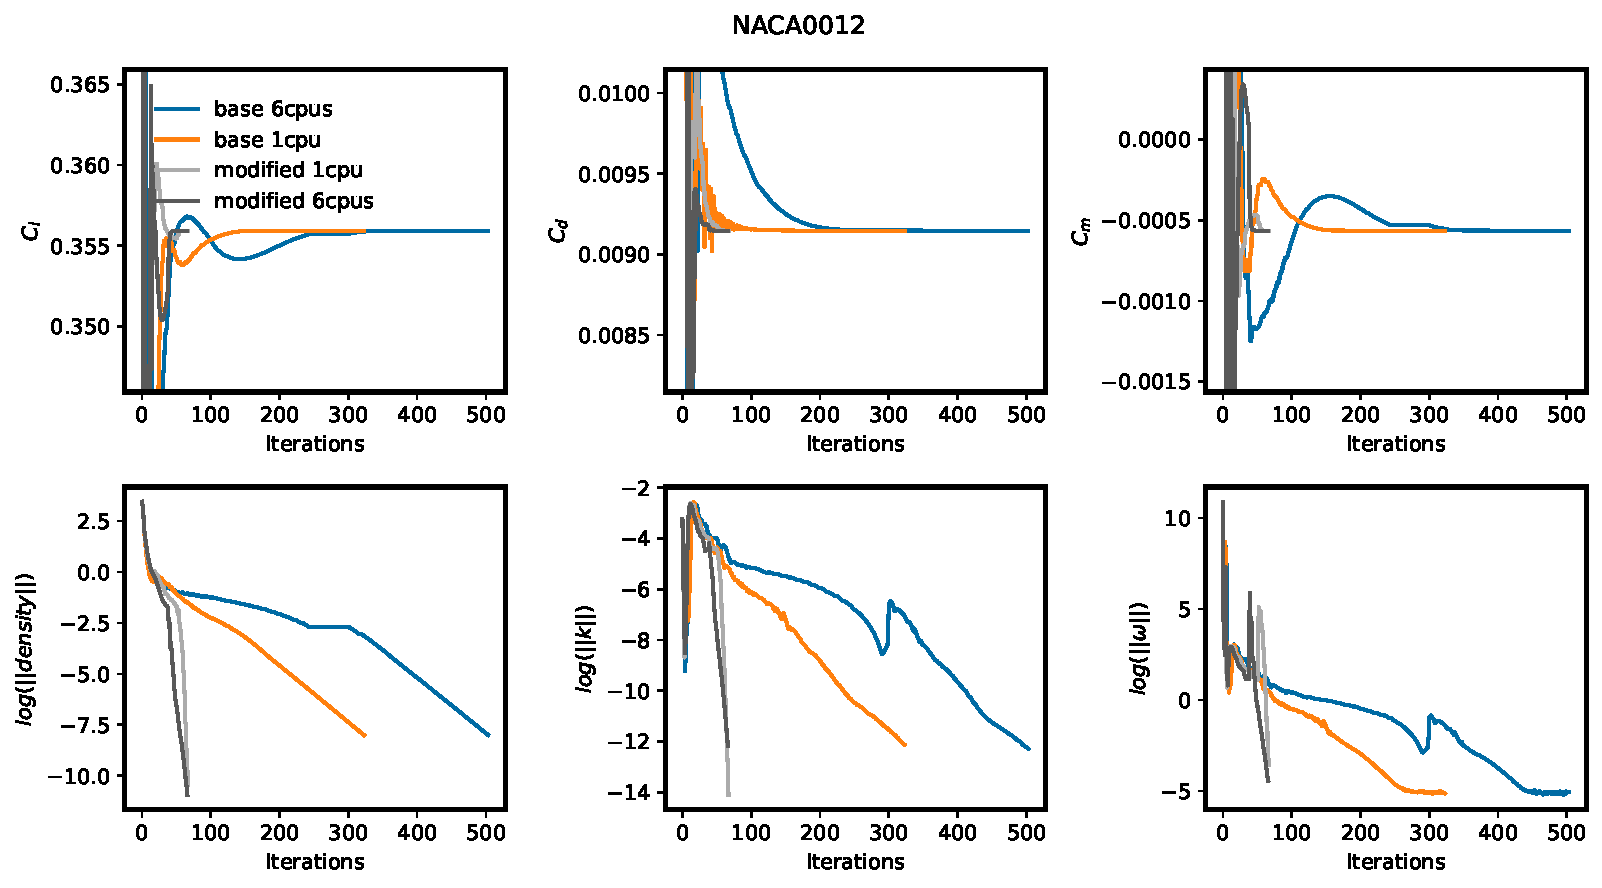
\includegraphics[width=1.0\textwidth]{plots/sc_NACA0012}
    \caption{Convergence history for NACA0012 testcase.}
    \label{fig:sc_NACA0012}
\end{figure}

\noindent Lets take a look at the baseline implementation first. It was
obtained using the ANK solver and a decoupled DADI solver for the turbulence
model. For the turbulence model, a total of 20 sub iterations were used. When
looking at the functions values (top row), it can be seen that 1 and 6 cpus
reach the same value. But 6 cpus need more iterations. It is not quite clear
what causes this, but it is a known phenomenon for low cpu counts and vanishes
when this number is increased. Production runs usually require tens or even
hundrets of cpus and thus this is not considered detrimental.


Now, lets look at the modified curves. Here, SST was differentiated and the
turbulence ANK and fully coupled CANK solvers are available. Annectdotal
evidence suggest SST is highly non-linear. This is especially true for the
inital stages of convergence. Due to this\footnote{The author believes the ANK
solver does some finite-differencing for some terms under the hood.}, the
turbulence DADI solver is way more efficient early on. Thus, at the beginning,
the regular ANK solver with decoupled DADI was used. But once a relative
convergence of 1e-6 is reached, the second order coupled ANK (CSANK) is
engaged. Once it gets traction, it exhibits almost Newton-like convergence. The
number of cpus does not really affect the number of iterations needed. It is
also obvious that the modified version approaches the same function values as
the baseline implementation. 




\subsubsection{RAE2822}
Figure \ref{fig:sc_RAE2822} shows a similar convergence plot for the RAE2822
testcase. Once again, the baseline and modified version with each 1 and 6 cpus
is plotted. It is important to note that this case is somewhat hard as it lies
in the transsonic regimes where shocks appear. But at the same time, it is even
coarser than the naca case which makes it hard to resolve them properly.

\begin{figure}[H] \centering
    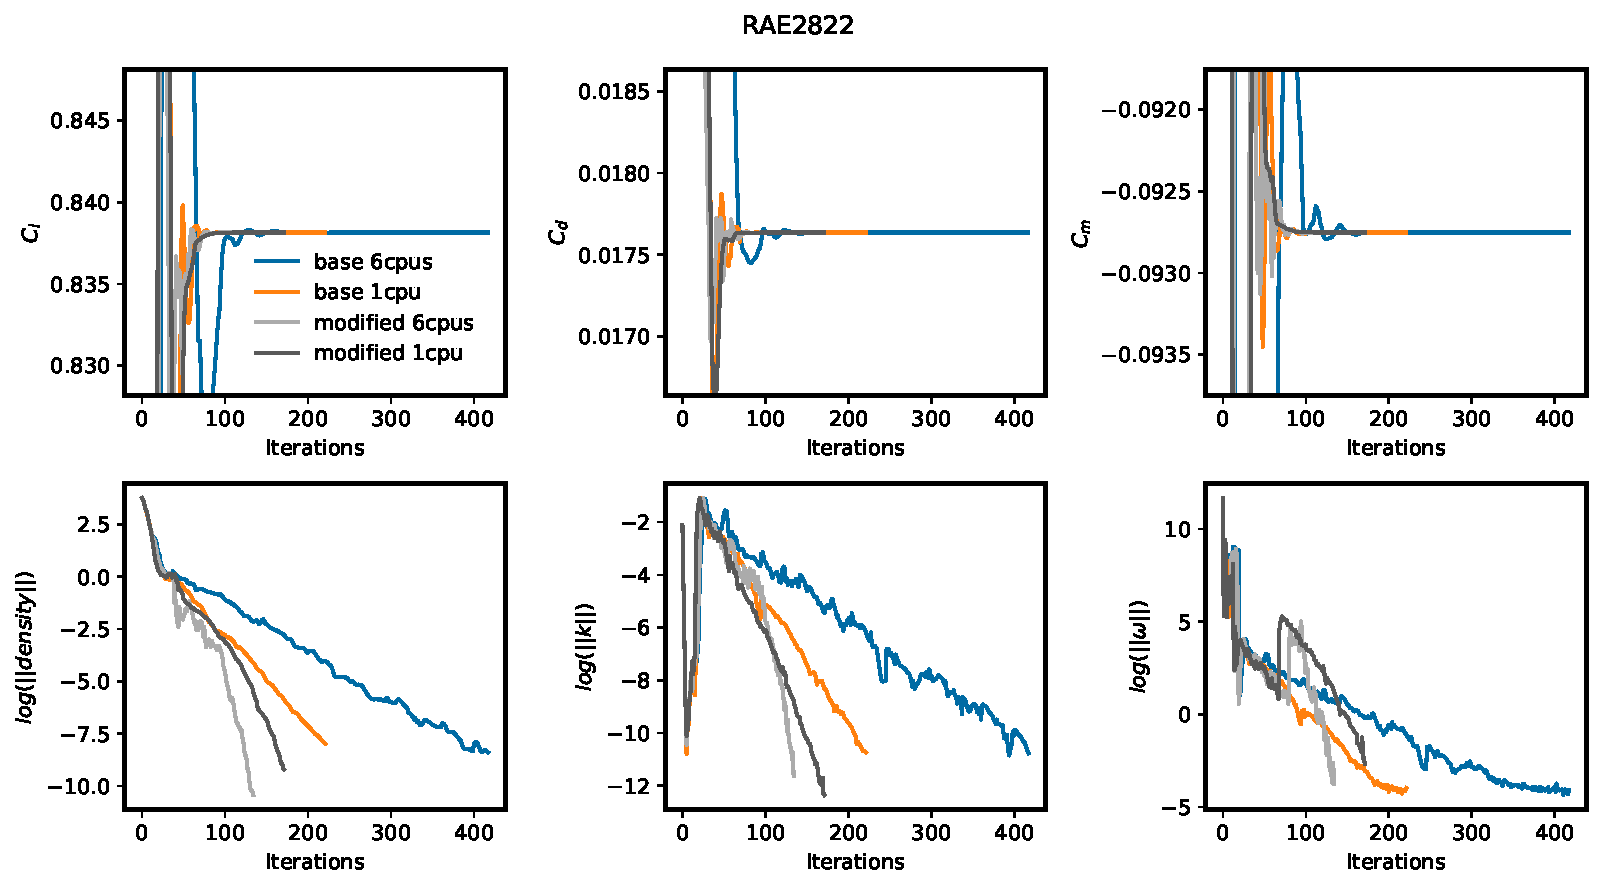
\includegraphics[width=1.0\textwidth]{plots/sc_RAE2822}
    \caption{Convergence history for RAE2822 testcase.}
    \label{fig:sc_RAE2822}
\end{figure}

\noindent First, lets glance ath the baseline. This has also been obtained
using the ANK solver for the flow variables and the DADI solver for the
decoupled turbulence variables. A similar pattern to the NACA
testcase appears: 1 cpu takes only half the iterations of what 6 cpus need.
But, the converged values are the same. When comparing the general line pattern
to the NACA testcase, it appears to be more 'wiggly' here. The author belieaves
this is due to the coarse mesh and transsonic regime. This probably increases
the sensitivity to the CFL number. During convergence, the ANK solver increases
the CFL number based on the current relative convergence. But the high
sensitivity makes the solver unstable and i starts to diverge. Once this is
detected, the CFL number is lowered again. Plese note that it is not as simples
as it seems here because the convergence of the linear system for the newton
step also influences the CFL number. The author just wants to stress that
probably some form of coupling causes the unsteady behavior. This should be
avoidable, but maybe more tuning or even a change to the CFL-ramping algorithm
is needed.

When looking at the modified version, a similar picture to NACA emerges. The
strategy was the same, first use ANK with DADI and once a relative convergence
of 1e-6 is reached, the CSANK solver is enganged which shows almost Newton-type
convergence. Although the contrast is not as big. But it also has to be noted
that that the before mentioned CFL dependence played a role here and some
parameters had to be clipped to increase robustness at the cost of convergence.





\section{Grid Convergence}
Figure \ref{fig:gc_2d_bump} shows the grid convergence for the 2d bump testcase
compared to data from the \textit{CFL3D} and \textit{FUN3D} CFD solvers. At
first glace, ADflow seems to be in the right bulk part but does not completely
agree with the reference. This difference may be explained through slightly
different model formulations. The turbulence production term used in ADflow is
called \textit{strain}. The author tried to converge the same case using the
\textit{vorticity} formulation but was unable to so. The reference data was
obtained using the \textit{SSTm} formulation. It is also possible that ADflow
uses a slightly different version.

\begin{figure}[H] \centering
    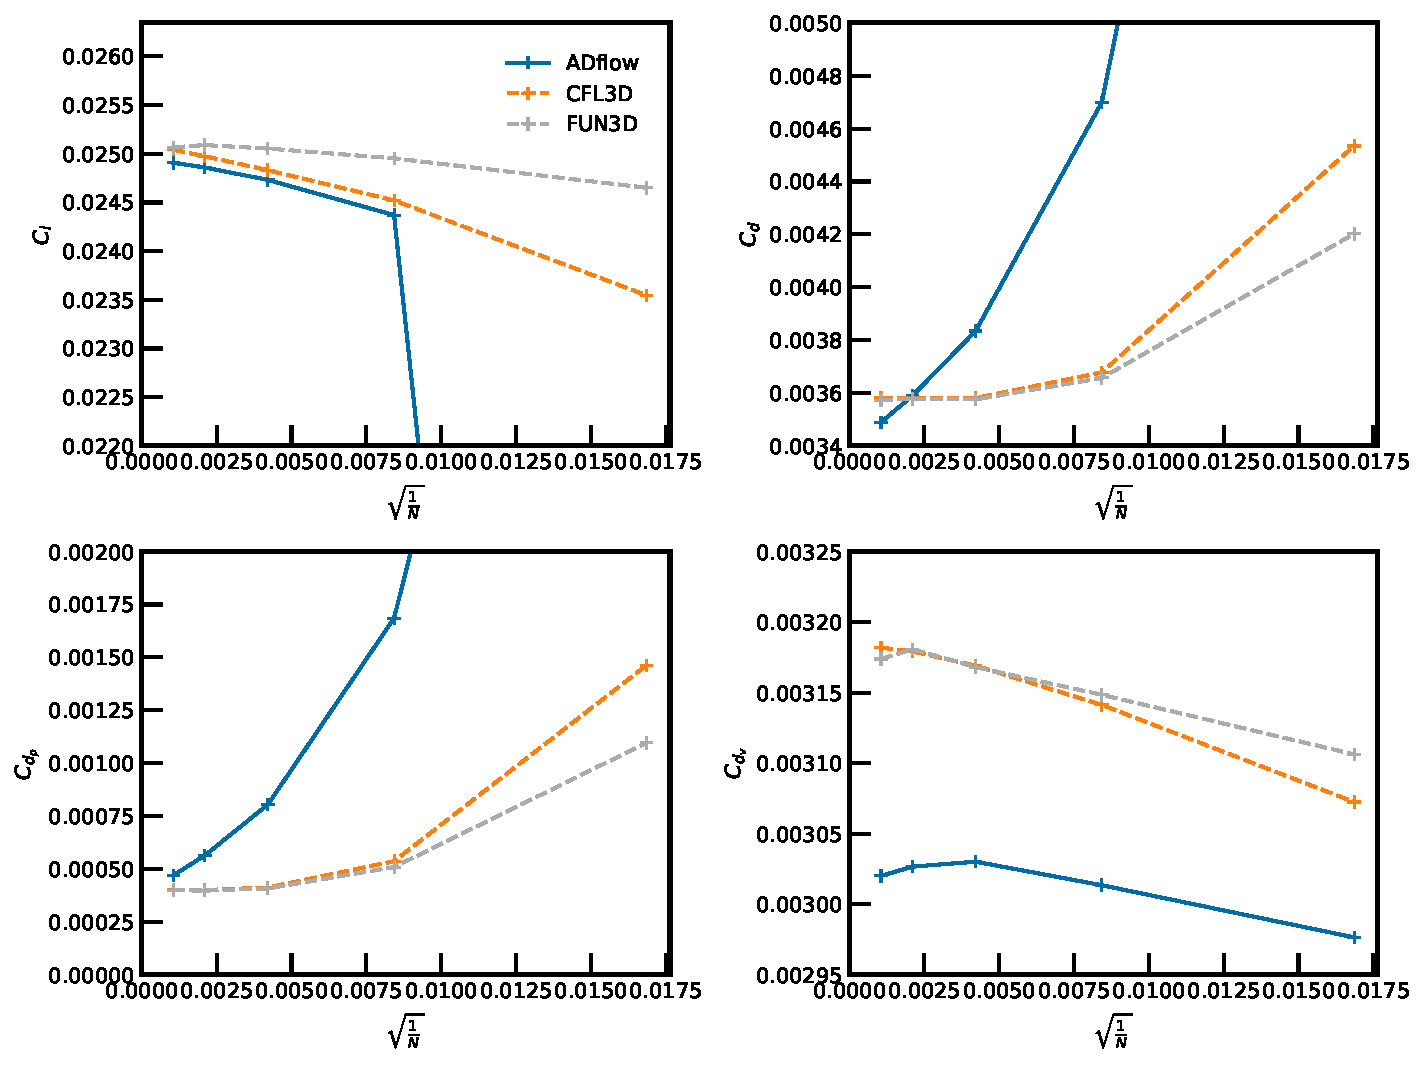
\includegraphics[width=1.0\textwidth]{plots/gc_2d_bump_nan-fix}
    \caption{Grid convergence for 2D bump. Reference data is from
    \cite{nasatmr}.}
    \label{fig:gc_2d_bump}
\end{figure}

\noindent But ignoring the discrepancies, the values seem to approach a certain
value which is desired.








\section{Partial derivatives}
\subsubsection{Forward mode}
To verify the forward partial derivatives, the 3D test case is first converged
to a relative tolerance of $1e-14$.\footnote{In theory, the partials should be
accurate regardless of the current convergence. But it is more valuable when
one can show that they are accurate for a converged state as this is what we
are after. } Once this is the case, the partials are compared against finite
difference and complex step. Anecdotal evidence suggest SST is highly
non-linear which is reflected in the fact that the FD partials are quite off
compared to AD. Table \ref{tab:partials_forward} lists the derivatives with the
relative accuracy compared to CS (stepsize was $1e-40$). Please not that the
tolerances had to be lifted partly to $1-e9$ instead of $1-e10$. This also
indicates that SST is highly non-linear.

\begin{table}[H]
    \centering
    \begin{tabular}{l r}
        \toprule
        Derivative                          & Relative tolerance \\
        \toprule
        $\partial R / \partial u$           & $\leq 1e-9$ \\
        $\partial f / \partial u$           & $\leq 1e-9$ \\
        $\partial F / \partial u$           & $\leq 1e-9$ \\
        \midrule
        $\partial R / \partial x_{geo}$     & $\leq 1e-9$ \\
        $\partial f / \partial x_{geo}$     & $\leq 1e-9$ \\
        $\partial F / \partial x_{geo}$     & $\leq 1e-9$ \\
        \midrule
        $\partial R / \partial x_{aero}$    & $\leq 1e-10$ \\
        $\partial f / \partial x_{aero}$    & $\leq 1e-10$ \\
        $\partial F / \partial x_{aero}$    & $\leq 1e-10$ \\
        \bottomrule
    \end{tabular}
    \caption{Relative accuracy of forward AD partials compared to CS.}
    \label{tab:partials_forward}
\end{table}


\subsubsection{Reverse mode}
To verify the backwards partials, a dot-product test was performed. Table
\ref{tab:partials_dotproduct_test} lists the tests  with the relative tolerance
it was passed. The only test that did not pass was $u \rightarrow F$. As $F$
are the nodal forces, those derivatives are only needed for aerostructural
optimization. The reason for failing is probably the fact, that those routines
buffer some values without recomputing. The changes to the wall distance
probably require changes to those routines as well. Because this was not done,
the test fails.

\begin{table}[H]
    \centering
    \begin{tabular}{l r}
        \toprule
        Dot product test                     & Relative tolerance \\
        \toprule
        $u \rightarrow R$                   & $\leq 1e-10$ \\
        $u \rightarrow F$                   & $\textcolor{red}{= 2e-6}$ \\
        \midrule
        $x_{geo} \rightarrow R$             & $\leq 1e-9$ \\
        $x_{geo} \rightarrow F$             & $\leq 1e-10$ \\
        \midrule
        $(u, x_{geo}) \rightarrow (du, F)$  & $\leq 1e-10$ \\
        \bottomrule
    \end{tabular}
    \caption{Relative accuracy of dot product test between forwards and
    backwards partial derivatives.}
    \label{tab:partials_dotproduct_test}
\end{table}


\subsubsection{Reverse\_fast mode}
The reverse\_fast partials are simply compared to the forwards routines. This
is possible because the first one is a subset of the former one. Table
\ref{tab:partials_fast} lists the relative accuracy. It obviously does not
agree at all. This is due to time constraints as the author could not proceed
to improve it further. But the fact that it yields a number and does not simply
crash is already an achievement.

\begin{table}[H]
    \centering
    \begin{tabular}{l r}
        \toprule
        backwards vs backwards\_fast        & Relative tolerance \\
        \toprule
        $u$                                 & $\textcolor{red}{= 5.7e4}$ \\
        \bottomrule
    \end{tabular}
    \caption{Relative accuracy of backwards\_fast routines compared to
    backwards.}
    \label{tab:partials_fast}
\end{table}







\section{Total derivatives}
As described in sec. XXX, the total derivatives were verified by comparing them
to complex step. As described in sec. XXX, ADflow may assemble the adjoint
system using either the forwards partials or the reverse\_fast partials. Table
\ref{tab:total_derivs} lists the relative difference of various methods
against complex step with a stepsize of $1e-200$.

\begin{table}[H]
    \centering
    \begin{tabular}{l r r r r}
        \toprule
        Name        & cmplx. ($h=1e-40$)   & adj. frwd. 1cpu           & 
            adj. frwd. 6 cpus         & adj. rev. fast 6 cpus    \\
        \toprule
        alpha       & -1.3e-09             & -5.3e-06                  & 
            -5.3e-06                  & \textcolor{red}{-8.0e-03} \\
        mach        & -6.1e-08             &  2.3e-05                  &  
            2.3e-05                  & \textcolor{red}{ 2.3e-01} \\
        \midrule
        span \#0    & -2.0e-09             &\textcolor{red}{ 4.0e-04}  &
            \textcolor{red}{-9.0e-04}  & \textcolor{red}{-1.0e-02} \\        
        twist \#0   &  9.3e-09             &\textcolor{red}{-1.0e-03}  &
            9.6e-05                    & \textcolor{red}{-1.4e-02} \\        
        shape \#0   & -5.3e-07             &\textcolor{red}{ 5.8e-02}  &
            \textcolor{red}{ 5.6e-02}  & \textcolor{red}{ 1.2e-00} \\         
        \bottomrule
    \end{tabular}
    \caption{Relative difference of gradients compared to compplex step
    (stepsize = 1e-200). The function of interest is $C_l$. When the DVs are a
    vector (e.g span), only the first variable is listed.}
    \label{tab:total_derivs}
\end{table}

\noindent First, lets look at the forward routines with 1 and 6 cpus. The first
two variables are \textit{aerodynamic}, meaning do not control the geometry. It
appears that they stay the same on 1 or 6 cpus. Their relative accuracy is
approx 1e-5. This is relatively low, but may be explained through the high
non-linearity of SST. It is also important to realize that those are the first
tries. This means, there will probably be better options and/or methods and
thus a higher accuracy should be expected in the future. When looking at the
\textit{geometric} derivatives, it becomes clear that they differ with the
number of cpus. Also the are less accurate than the geometric ones. This
probably indicates a problem with modification done to the wall distance
exchange routines. This should be fixable with only a bit more time.

As already indicated with the partial reverse\_fast routines, the total
derivatives are also completely wrong. But once again, the fact that a number
was obtainable is already an achievement. This should also be fixable and only
needs a bit more time.








\section{Summary}
The results show that a prototype state was achived. SST does converge using
the coupled ANK solver and also gradients can be obtained. But of course, there
are still some bugs present. Some other results were more anecdotal and could
not be proven properly. The following list shows the insights gained through
this project.

\begin{itemize}
    \item SST is probably highly non-linear.

    \item ANK does work using the AD preconditioner. But sometimes NaNs appear.

    \item ANK does not work using FD preconditioner (probably due high
        non-lineary of SST).

    \item Physicality check for ANK needs to be adjusted to SST.

    \item Prototype adjoint is running.

    \item Aerodynamic derivatives using forward routines are accurate.

    \item Geometric derivatives using forward routines are not accurate.

    \item There is probably a bug in the halo exchange of the wall distance in
        the backwards routines.

    \item Derivatives using reverse\_fast routines are not accurate at all.

    \item SST appears to be implemented correctly.
\end{itemize}
